\documentclass[12pt, a4paper]{article}
\usepackage[margin=2 cm]{geometry} % 上下左右距離邊緣2cm
\usepackage{amsmath,amsthm,amssymb,amsbsy} % 引入 AMS 數學環境
%\usepackage{newtxmath,newtxtext} %Times new Roman 來源
\usepackage{fontspec}
\usepackage{graphicx}    % 圖形插入用
\usepackage{float}       % 浮動環境
%\usepackage{subfig}      % subfigures
\usepackage{subcaption}
\usepackage{type1cm}	 % 設定fontsize用
\usepackage{titlesec}   % 設定section等的字體
\usepackage{titling}    % 加強 title 功能
\usepackage{fancyhdr}   % 頁首頁尾
\usepackage{bm}
\usepackage[square, comma, numbers, super, sort&compress]{natbib}
\usepackage[unicode=true, pdfborder={0 0 0}, bookmarksdepth=-1]{hyperref}
\usepackage{pgf,tikz}
\usepackage{mathrsfs}
\usepackage{datetime}
\usepackage{physics}
\usepackage{sectsty}
\sectionfont{\fontsize{16}{15}\selectfont}
\subsectionfont{\fontsize{14}{15}\selectfont}
\usdate
\linespread{1.2}
\usepackage{xeCJK}  % xelatex 中文
\setmainfont{Times New Roman}
\newCJKfontfamily\Kai{標楷體}
\setCJKmainfont[AutoFakeBold=3,AutoFakeSlant=.4]{標楷體}
\XeTeXlinebreaklocale "zh"            
\XeTeXlinebreakskip = 0pt plus 1pt
\usepackage{ruby}
\setlength{\headheight}{15pt}  %with titling
\setlength{\droptitle}{-1.5cm} %title 與上緣的間距
\parindent=24pt %設定縮排的距
\usepackage{array}
\renewcommand{\proofname}{\bf Proof: } %修改Proof 標頭
\newtheoremstyle{mystyle}% 自定義Style
  {6pt}{15pt}%       上下間距
  {}%               內文字體
  {}%               縮排
  {\bf}%            標頭字體
  {.}%              標頭後標點
  {1em}%            內文與標頭距離
  {}%               Theorem head spec (can be left empty, meaning 'normal')
% 改用粗體,預設 remark style 是斜體:
\theoremstyle{mystyle}	% 定理環境Style

\usepackage{tikz}
\usetikzlibrary{shapes.geometric, arrows}

\tikzstyle{startstop} = [rectangle, rounded corners, minimum width=5cm, minimum height=1cm,text centered, draw=black, fill=red!30]
\tikzstyle{process} = [rectangle, minimum width=5cm, minimum height=1cm, text centered, draw=black, fill=blue!30]
\tikzstyle{decision} = [diamond, minimum width=3cm, minimum height=1cm, text centered, draw=black, fill=green!30]
\tikzstyle{arrow} = [thick,->,>=stealth]

%%%%%%%%%%%%%%%%%%defnple
\newtheorem{ex}{Example}
\newtheorem{pr}{Problem}
\newtheorem{df}{Definition}
\newtheorem{thr}{Theorem}
\newtheorem{pp}{Property}

\pagestyle{fancy}
\fancyhf{}
\fancyhead[L]{蔡杰達}
\fancyhead[R]{雲物理加分作業}
\fancyfoot[R]{\thepage}

\begin{document}
\renewcommand{\headrulewidth}{0.4pt}
\begin{center}
\begin{Large}
\textbf{泊松方程與水物成長}
\end{Large}
~\\
~\\
蔡杰達
\end{center}
\section{簡介}
在課堂中,我們曾經提過可以將水氣的空間分佈寫成泊松方程(Poisson eqn.),同時這也是靜電學的基礎。在本篇文章中,首先我們會利用電磁學的一些結果去詮釋水氣分佈的狀況,包括解釋冰晶靜電容的原理以及冰晶凝華成長的狀況,再來利用數值方法去處理冰晶凝華成長。

\section{數學表述}
在課堂中,我們利用了兩式子描述的水氣的時空分佈。
\begin{align}
    \pdv{\rho}{t} + \div{J} &= 0 \\
    J = -D\gradient{&\rho}
\end{align}
第一條為質量守恆方程,第二條為Fick's First Law。將第二條帶入第一條後可以看到
\begin{equation}
    \pdv{\rho}{t} = D\laplacian{\rho}
\end{equation}
這同時也是Fick's Second Law。而我們通常會做準靜態的假設,意即
\begin{equation}
    \pdv{\rho}{t} = 0, \laplacian \rho = 0
\end{equation}
但是這不可能為0,因為如果水氣與時間無關,則水滴或冰晶便不會成長,故我們稱之為準靜態假設。在此準靜態假設下,我們可以做出一些與電磁學的類比。首先我們可以發現電位\(V\)可以直接類比為水氣濃度\(\rho\),故之前課堂上才會得到\(\rho \propto 1/r\)。接著我們觀察到\(J = -\grad{\rho}\),這同樣也對比到\(E = -\grad{V}\),可以發現電場\(E\)可以直接類比為水氣通量\(J\)。若我們想計算單位時間內通過某封閉表面的水氣量,即凝結的量,我們可以做\( \dv{m}{t} = \oint J \dd A\)。同樣的在電磁學當中,我們可以做的是\(q = \oint E \dd A\)。從這我們可以將電荷\(q\)類比為該處的質量增加速率\(\dv{m}{t}\)。而為了維持我們準靜態的假設,我們必須保證質量增加速率都在邊界,在電磁學也有類似的事,便是我們考慮的電荷都發生在邊界上。惟與電磁學不同,電磁學中電荷是電位的source term,但這裡質量增加速率代表的是邊界條件的變化。\\
\\
在冰晶凝華成長中,課堂中曾經提到在尖端的成長速率會比其他地方快。而此現象可以利用尖端放電解釋。在電磁學中,一導體會最喜歡在尖端處累績電荷,並且在此放電。而對比到冰晶的情況,我們可以將冰晶類比成導體,而電荷類比成凝結速率。而我們有很好的理由可以將冰晶類比成導體,那就是冰晶表面是一個等水氣密度的邊界,而導體是一個等電位體。所以我們可以將尖端成長速率類比成尖端的電荷,因此便很好的解釋了尖端成長速率較其他地方來的快。在冰晶靜電容中,我們最想得到的是一個水氣密度和成長速率的關係式,亦即\(\dv{m}{t} = C \rho\)。對比到電磁學中,可以發現是\(q = CV\),發現是電磁學當中的電容。因此才會有冰晶靜電容是電容的這種類比。

\section{冰晶凝華數值計算}
我們可以利用電腦計算冰晶隨時間的成長過程。計算流程如下

\vspace{0.5 cm}
\begin{center}
\begin{tikzpicture}[node distance=2cm]
% Nodes
\node (step1) [process] {解水氣分佈};
\node (step2) [process, below of=step1] {計算梯度場};
\node (step3) [process, below of=step2] {解出暫時邊界分佈};
\node (step4) [process, below of=step3] {計算 concave hull};
\node (step5) [process, below of=step4] {估計表面融化};
\node (step6) [process, below of=step5] {解得新邊界分佈};

% Arrows
\draw [arrow] (step1) -- (step2);
\draw [arrow] (step2) -- (step3);
\draw [arrow] (step3) -- (step4);
\draw [arrow] (step4) -- (step5);
\draw [arrow] (step5) -- (step6);
\draw [arrow] (step6.east) -- ++(2,0) |- (step1.east);
\end{tikzpicture}
\end{center}
重複這個流程多次以後可以得到一段時間後的雪花成長。
\subsection{解水氣分佈}
本解將會將二維空間切成正方方格,為了維持精度,我們可以切成500\(\times \)500格。而要解出Poisson eqn.,我們採用Finite Difference Method。離散Laplacian可以表示如下
\begin{equation}
    \frac{(u_{x+\Delta x, y}-u_{x, y})}{\Delta x} - \frac{(u_{x, y}-u_{x - \Delta x, y})}{\Delta x} + \frac{(u_{x, y + \Delta y}-u_{x, y})}{\Delta y} - \frac{(u_{x, y}-u_{x, y - \Delta y})}{\Delta y} 
\end{equation}
由於是網格,我們讓\(x = i, y = j, \Delta x = \Delta y = 1\),原式變成
\begin{equation}
    \frac{1}{\Delta x^2} (u_{i+1,j} + u_{i-1,j} + u_{i,j+1} + u_{i,j-1} - 4 u_{ij}) = 0
\end{equation}
接下來我們要設定邊界條件,在冰晶的初始邊界條件是六邊形的邊界設成1,接下來就可以開始迭代並開始等待至收斂為止。
\subsection{邊界分佈}
而在解出水氣場後,我們可以計算邊界上的梯度場,而此處的梯度場就是此處的\(\dv{m}{t}\)。假設邊界點為\((x, y)\),則新邊界點為
\begin{equation}
    (x, y) \rightarrowtail (x, y) + (\grad{\rho} \cdot \hat{\vb{n}}) \hat{\vb{n}}
\end{equation}
而\(\hat{n}\)是邊界的法向量。\\
再來我們可以找出邊界的concave hull,便可以找出外邊界。找完外邊界以後便可以模擬融化的情況。在一般沒有融化的情況下,水氣都只會凝結在尖端,會變成很長的針狀結晶,若要有類似片狀成長則必須要讓他融化並附在表面上。而我們利用了幾種融化模型,包括Gaussian Convolution讓邊界模糊化,進而讓尖端不會過尖達到效果等。最後完成這些後即完成新的邊界迭代,並可進入下一輪計算。
\subsection{結果探討}
\subsubsection{水氣場分佈}
\begin{figure}[H]
\centering
\begin{subfigure}{.5\textwidth}
    \centering
    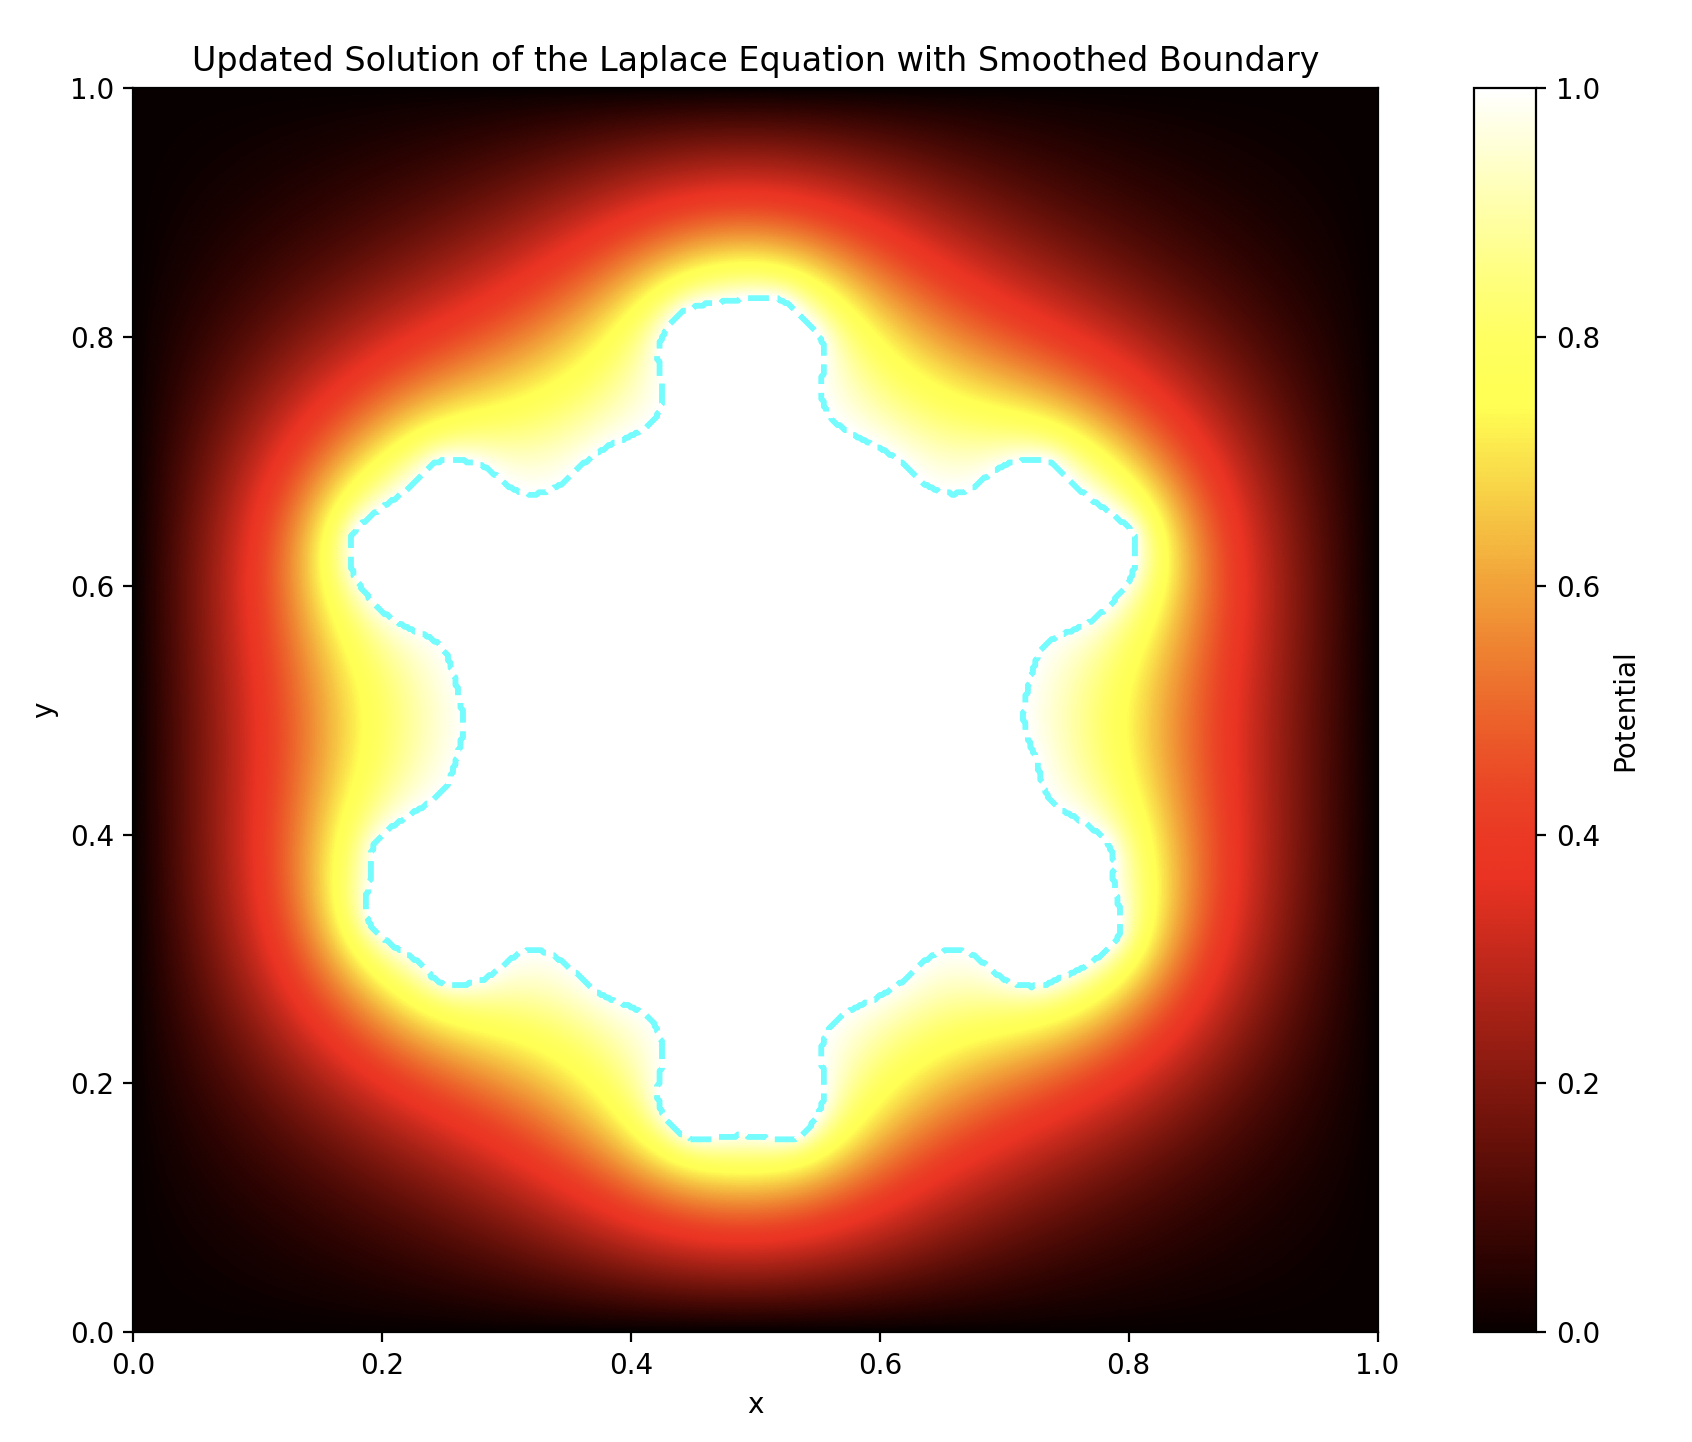
\includegraphics[height=.8\linewidth]{potential.png}
    \caption{水氣場分佈}
    \label{pot}
\end{subfigure}%
\begin{subfigure}{.5\textwidth}
    \centering
    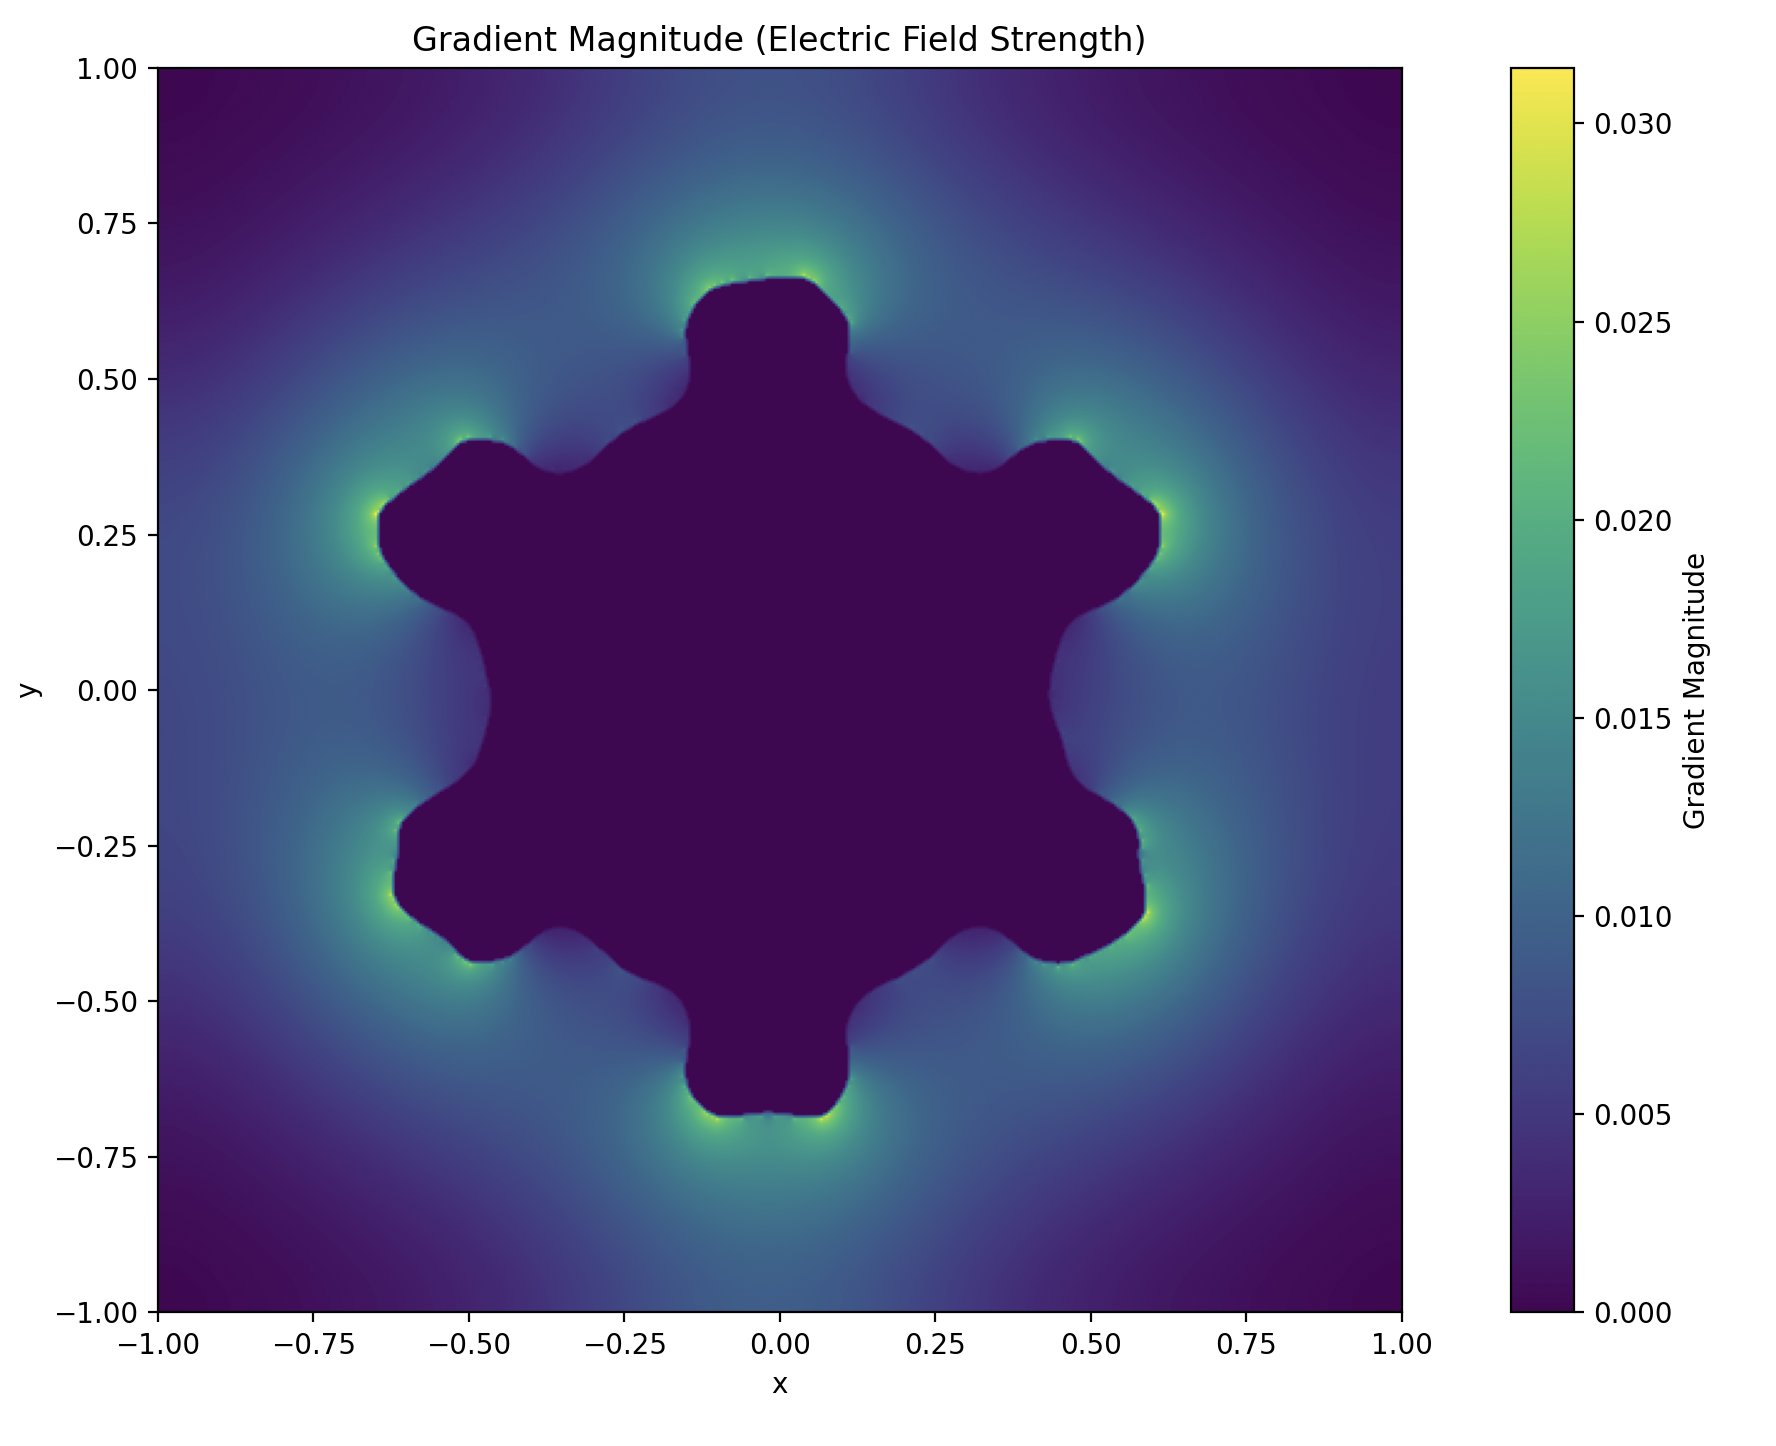
\includegraphics[height=.8\linewidth]{gradient.png}
    \caption{水氣通量大小分佈}
    \label{grad}
    \end{subfigure}
    \caption{水氣場與通量分佈}
    \label{pog}
\end{figure}
首先在水氣場分佈中的藍線是我們的邊界,在邊界內都是1,而在邊界外則由Poisson的解給定。可以觀察到此解是合理的,且解看起來並沒有不連續或者不平滑的現象發生。另外可以看到水氣在離邊界越遠會越與邊界形狀不敏感,也是符合預期。再來看到梯度場大小,可以看到在尖端的梯度非常的大,因此水氣通量會較大,因此尖端成長比較快。而在邊界內部則可以看到梯度都是0,因為邊界內都是定值1。除此之外在凹槽的地方都可以看見梯度是很小的,因此缺刻的地方只會繼續缺刻,而突出的地方則會突出更多。
\subsubsection{邊界分佈}
我們可以比較不同的邊界分佈情況。首先我們先觀察初始狀態,亦即沒有經過任何處理的暫時邊界分佈。
\begin{figure}[H]
    \centering
    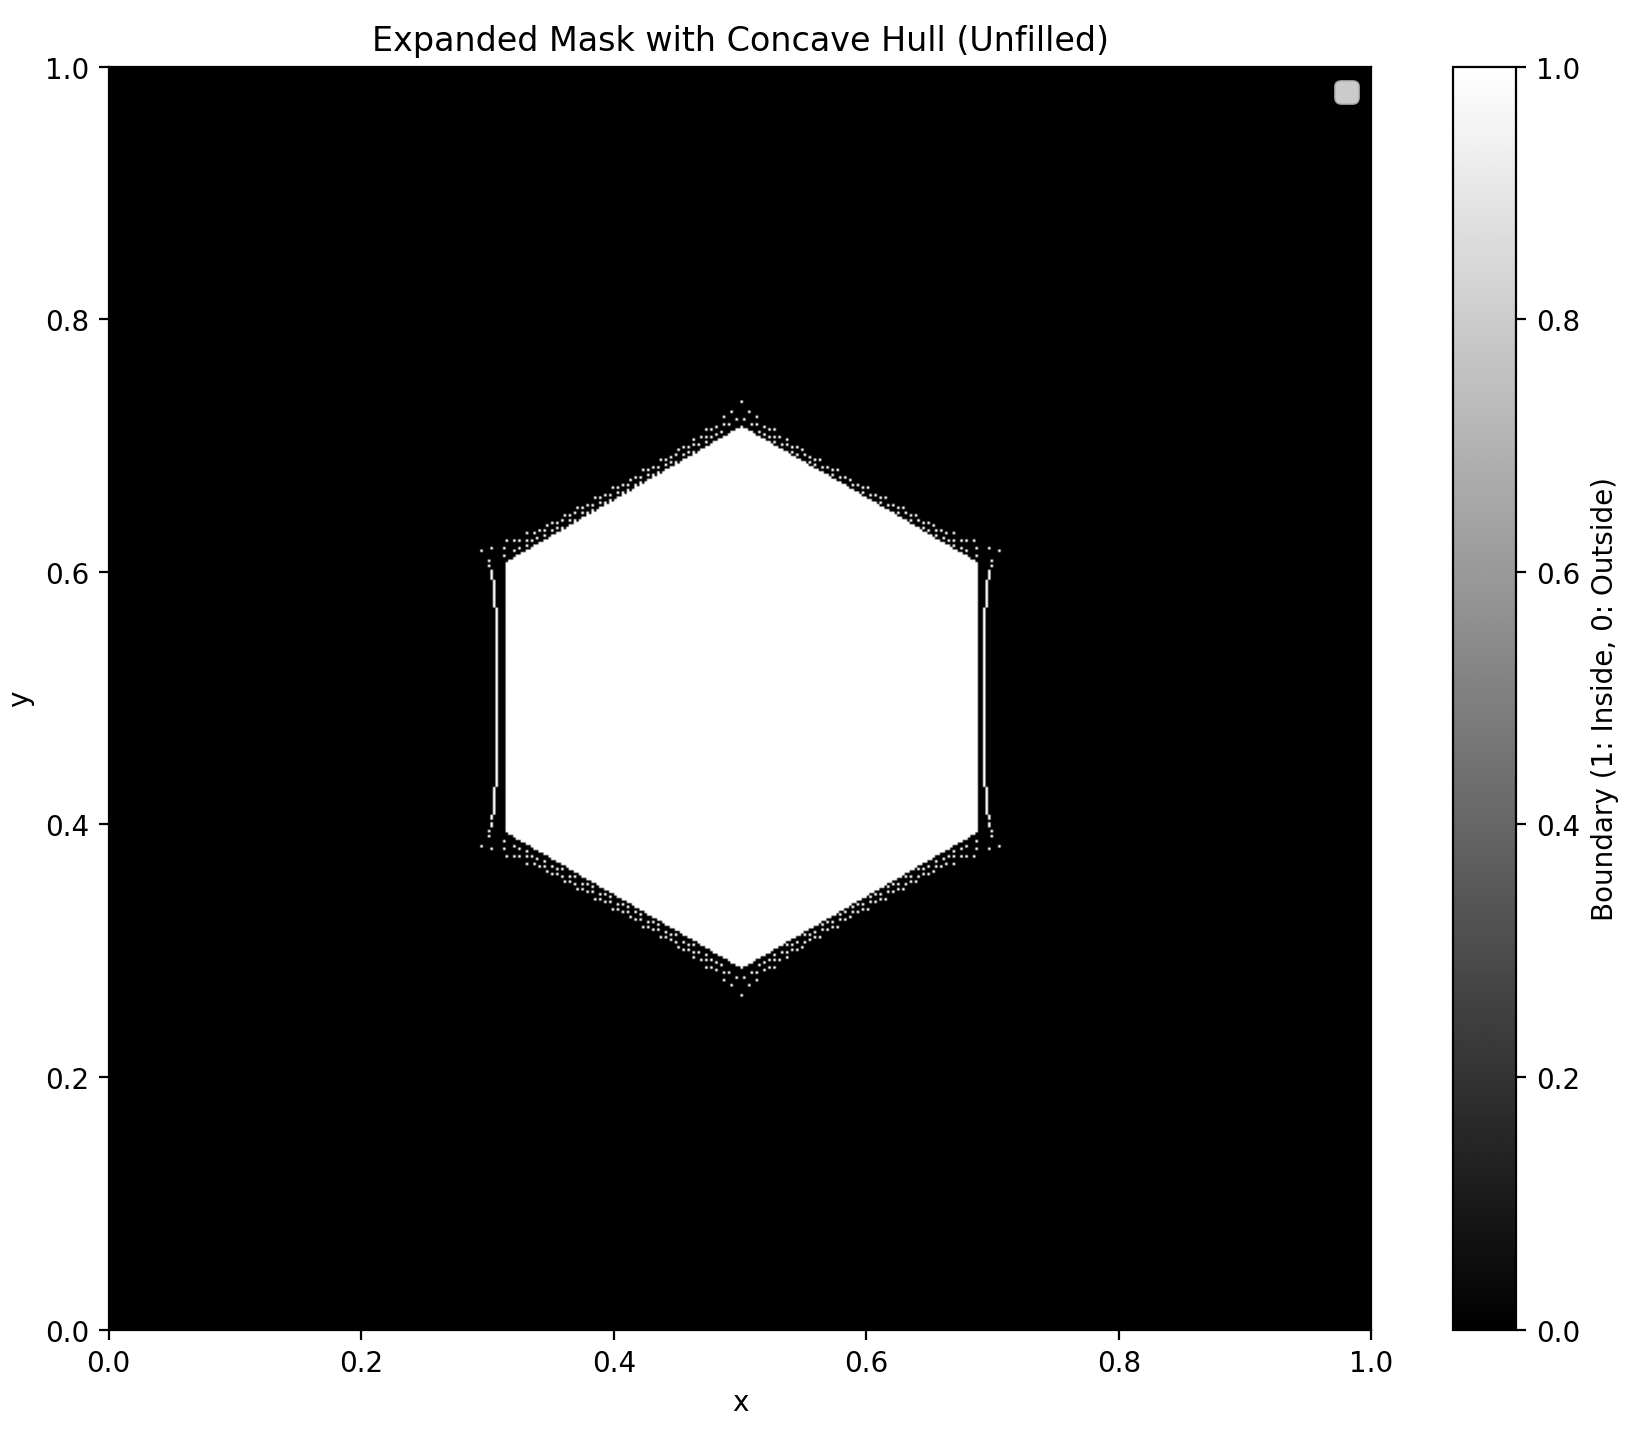
\includegraphics[width = 8 cm]{bad_boundary.png}
\end{figure}
從中可以看到若直接將邊界推出去會出現不連續的情況,因此如何將中間空缺的部分填滿是很重要的。我們可以計算外邊界的Concave Hull,再將Concave Hull 填滿,如下圖所示。而因為是取Concave Hull,故可以調整參數而改變最後Concave Hull的範圍。但是如果計算Concave Hull會讓我們的解析度下降,因為這樣才能找出外表面而不會太凹凸不平。雖然一般雪花也是凹凸不平的,但這個凹凸不平是不對稱的,所以是來自數值誤差。在下圖中我們可以比較不同參數給出的Concave Hull。
\begin{figure}[H]
\centering
\begin{subfigure}{.5\textwidth}
    \centering
    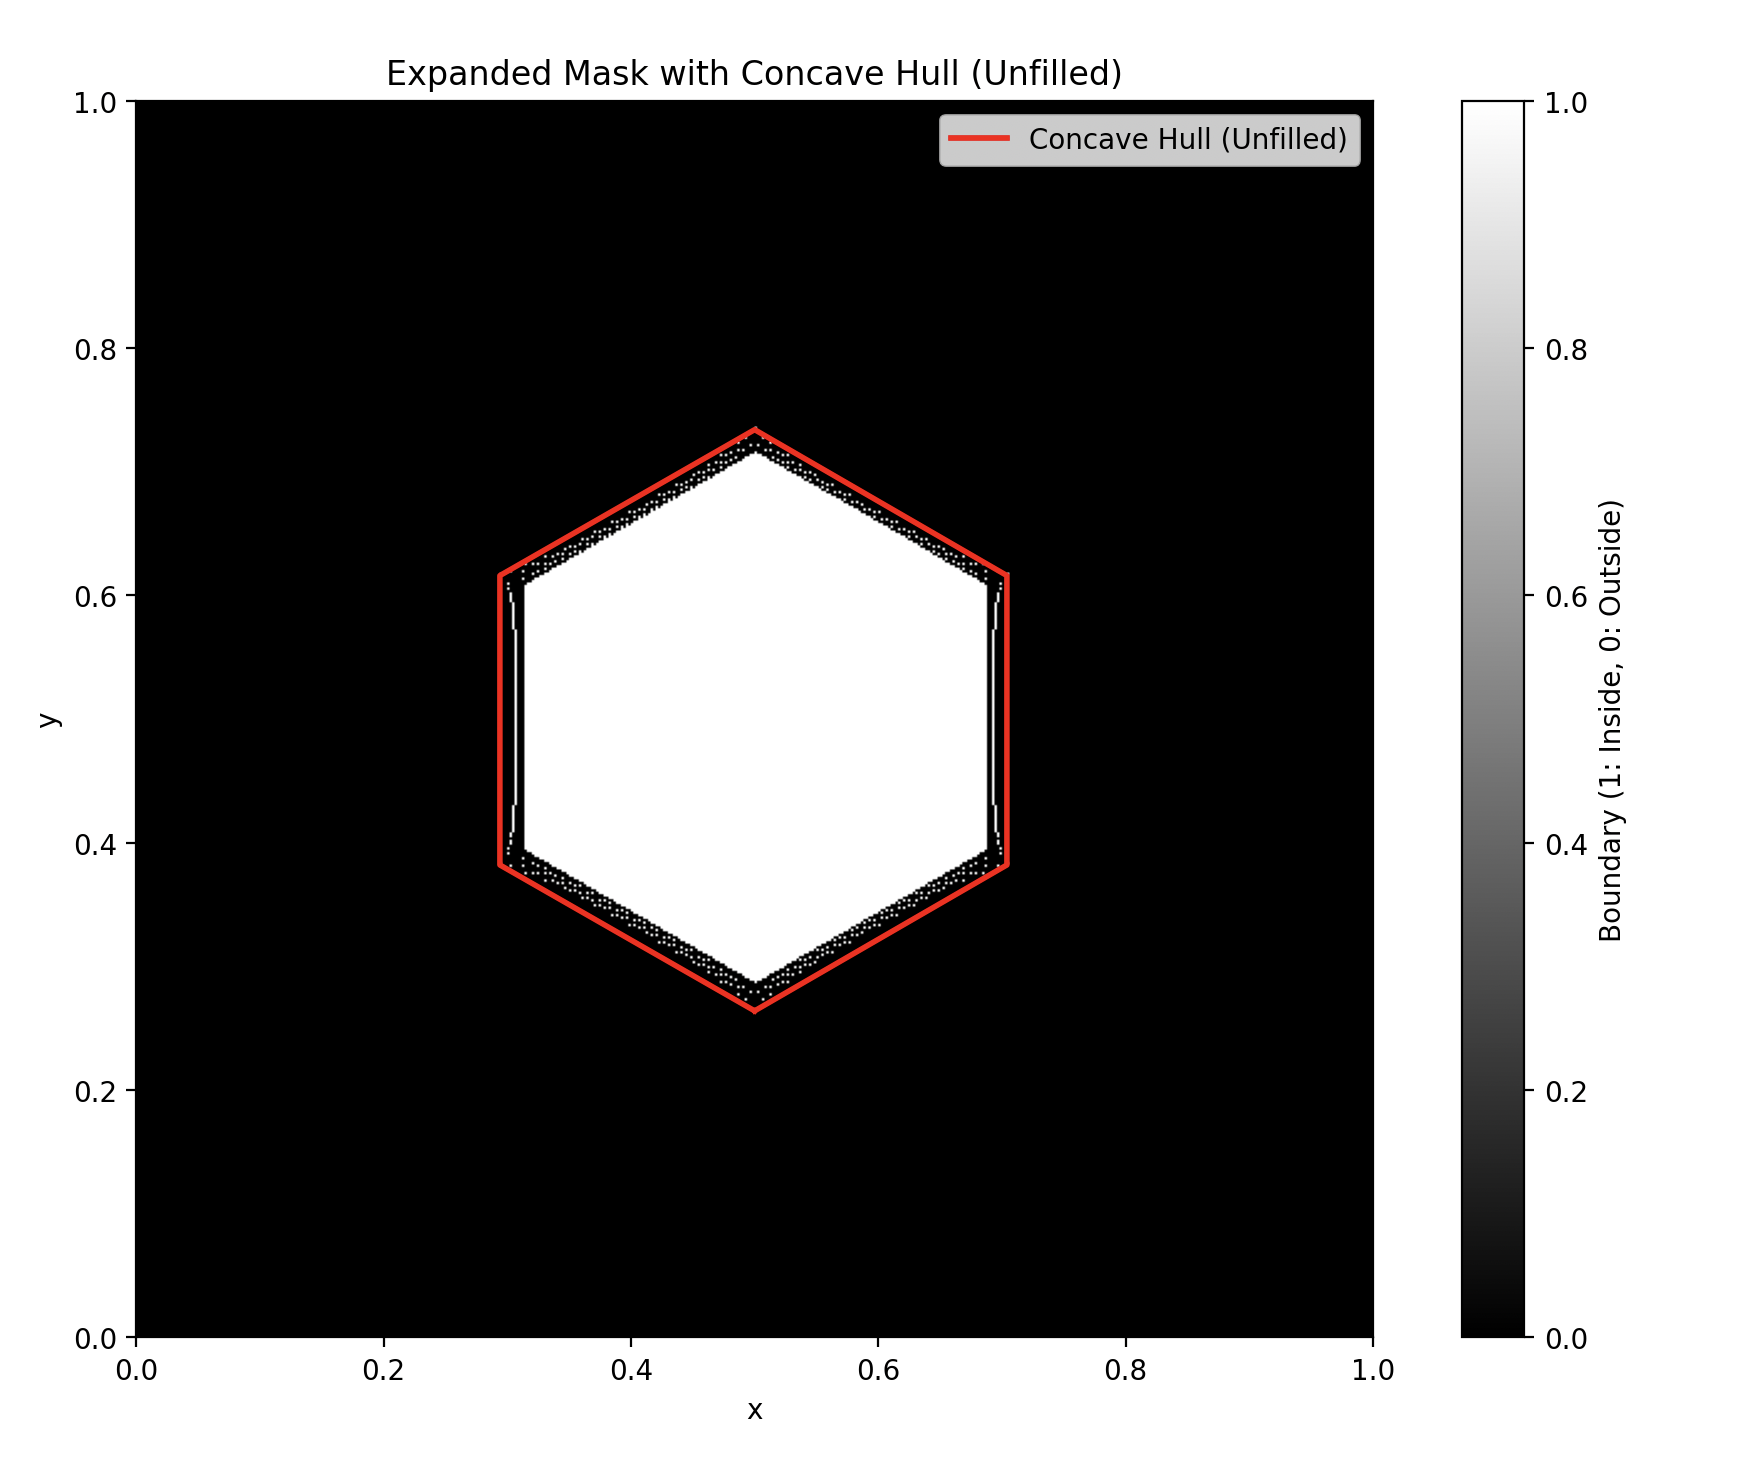
\includegraphics[height=.8\linewidth]{alpha_0.png}
    \caption{\(\alpha = 0\)}
    \label{pot}
\end{subfigure}%
\begin{subfigure}{.5\textwidth}
    \centering
    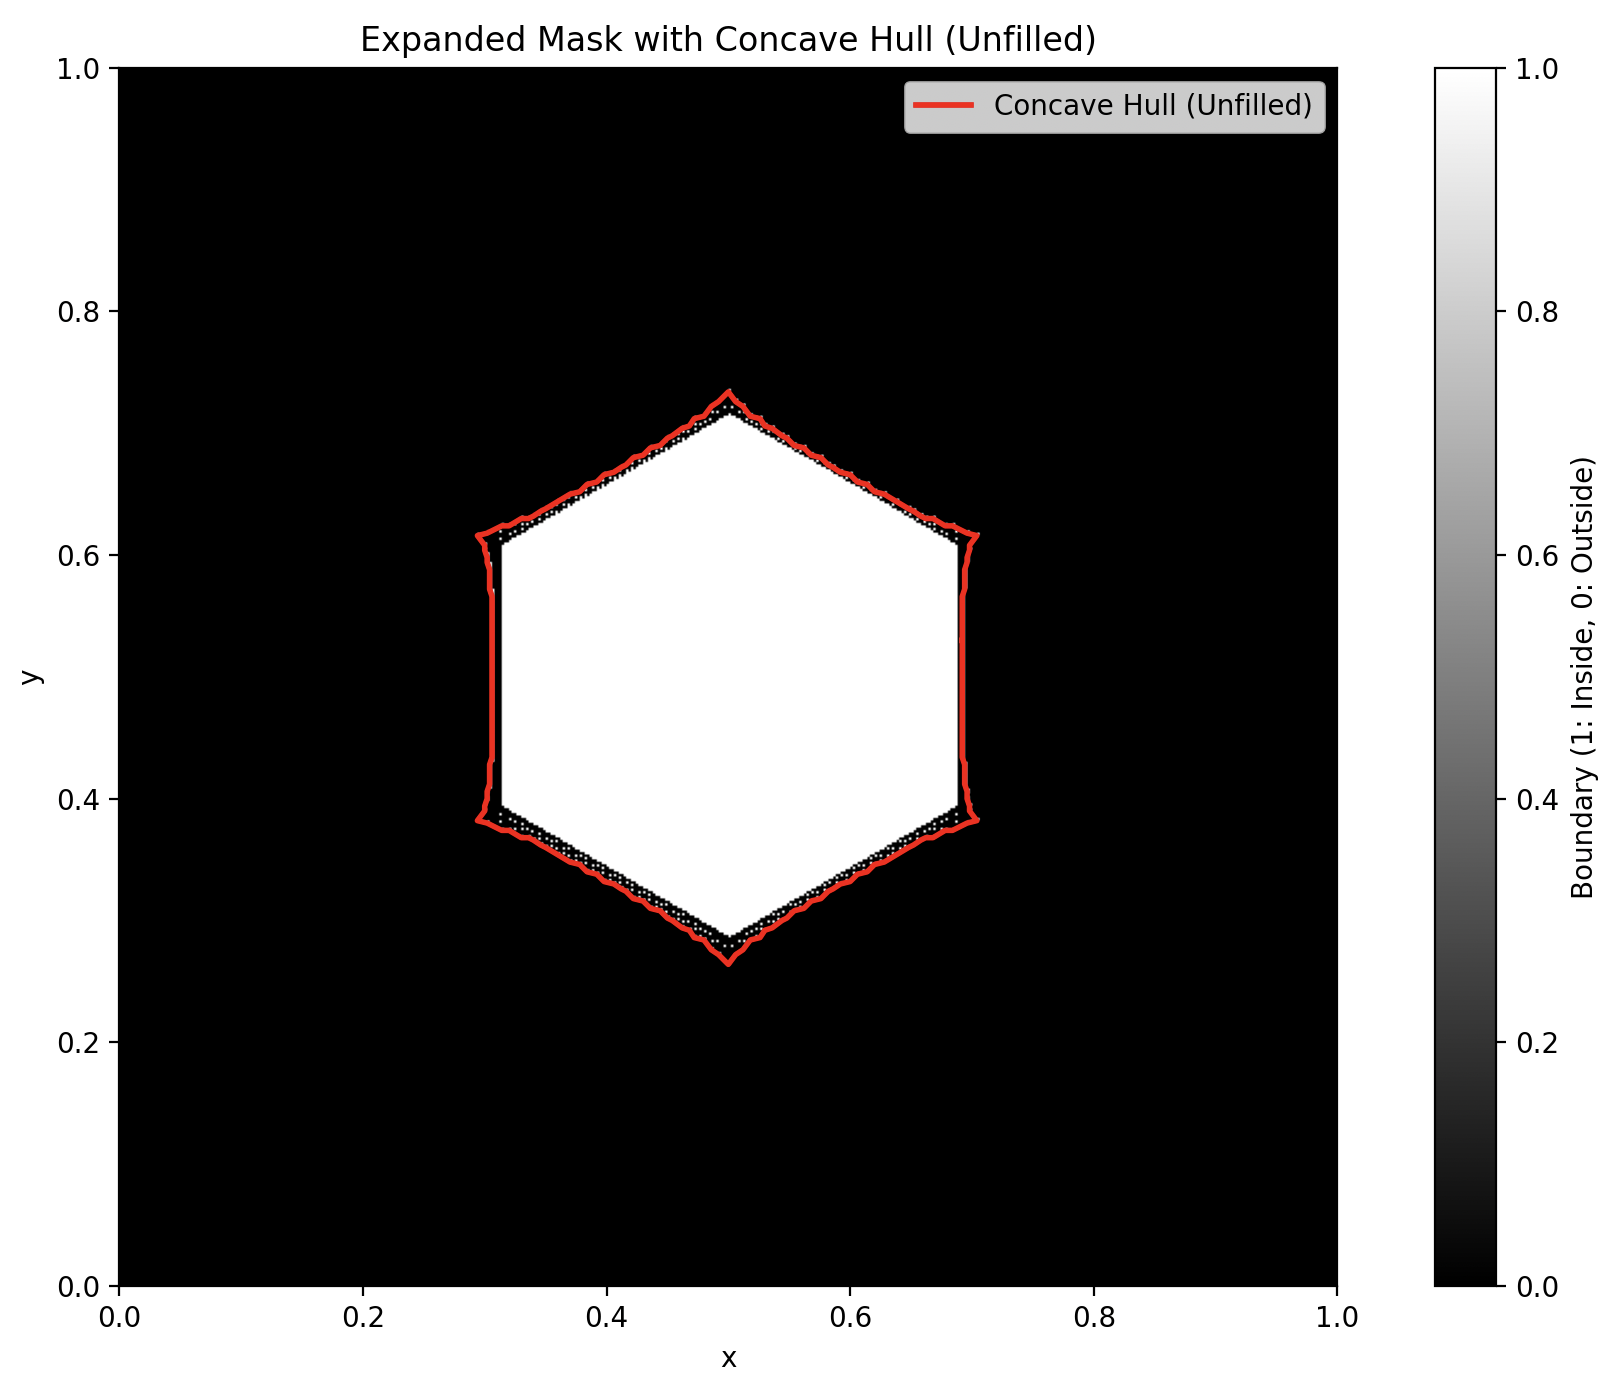
\includegraphics[height=.8\linewidth]{alpha_2.png}
    \caption{\(\alpha = 0.2\)}
    \label{grad}
    \end{subfigure}
    \caption{不同\(\alpha\)參數對邊界的改變}
    \label{pog}
\end{figure}
我們可以發現在\(\alpha = 0\)是做Convex Hull,負責把最外面的邊界找出來,而當有\(\alpha = 0.2\)時則可以找到比較貼切的邊界。
\subsubsection{融化模型}
融化模型總共有三種,第一種是假設邊界會變成液滴,因而成為具有半徑的球狀液滴,第二種是做Gaussian Convolution,讓邊界變得不會過尖而變得圓滑,第三種是超過某種水氣通量後便進行截斷,如大於0.020的水氣通量全部當0.020等。如此的好處是冰晶的成長會是片狀的,符合融化的特性。我們也同時比較沒有利用融化模型的狀況。
\begin{figure}[H]
\centering
\begin{subfigure}{.5\textwidth}
    \centering
    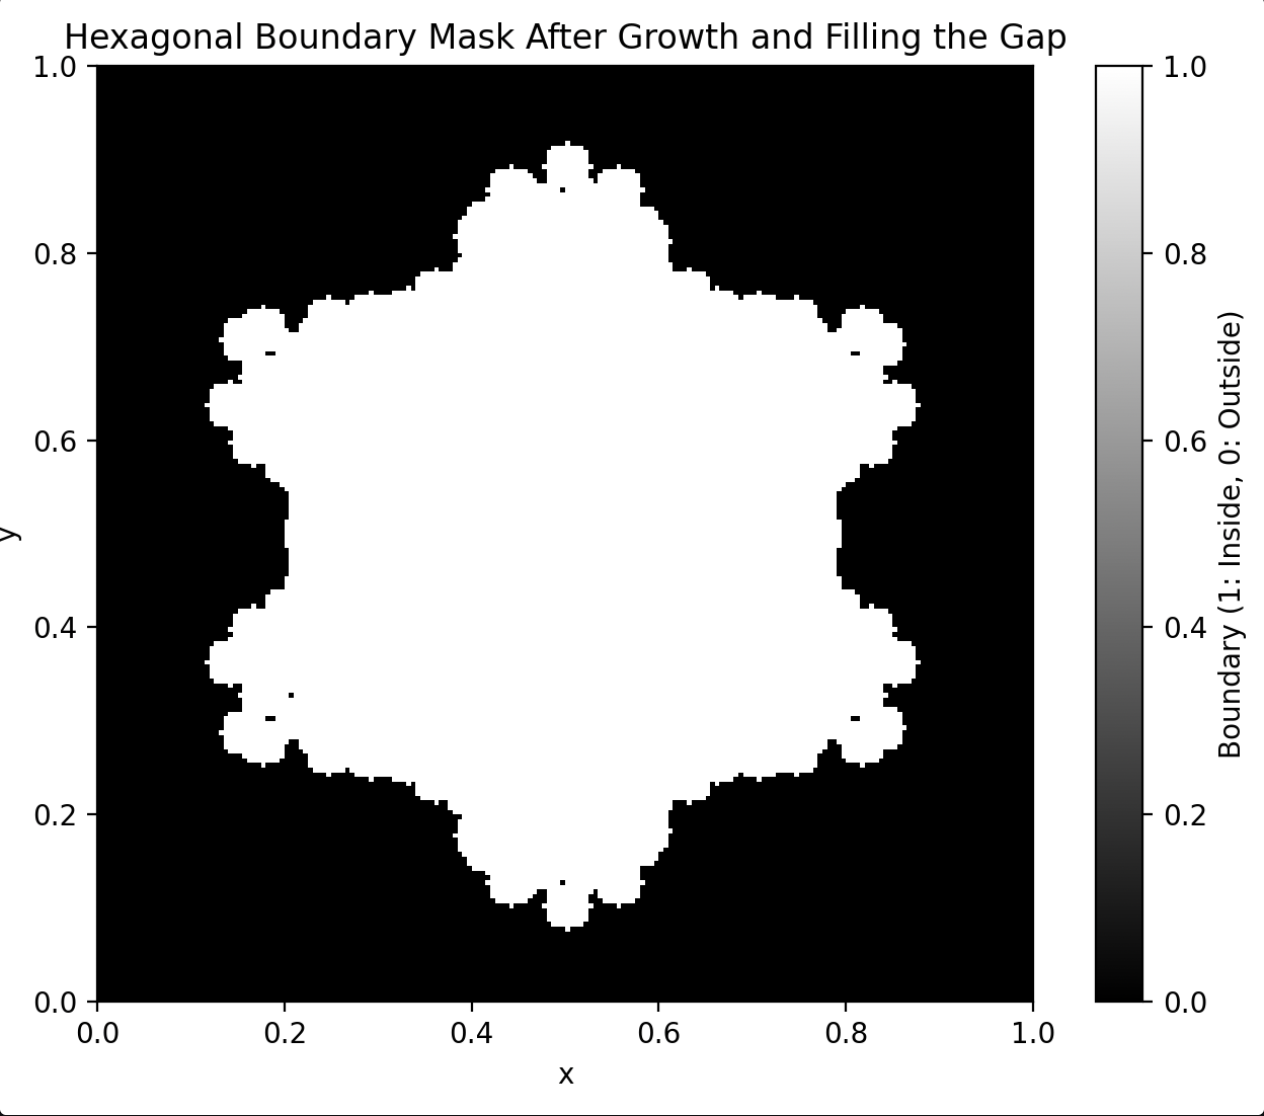
\includegraphics[height=.8\linewidth]{sphere.png}
    \caption{液滴法}
    \label{pot}
\end{subfigure}%
\begin{subfigure}{.5\textwidth}
    \centering
    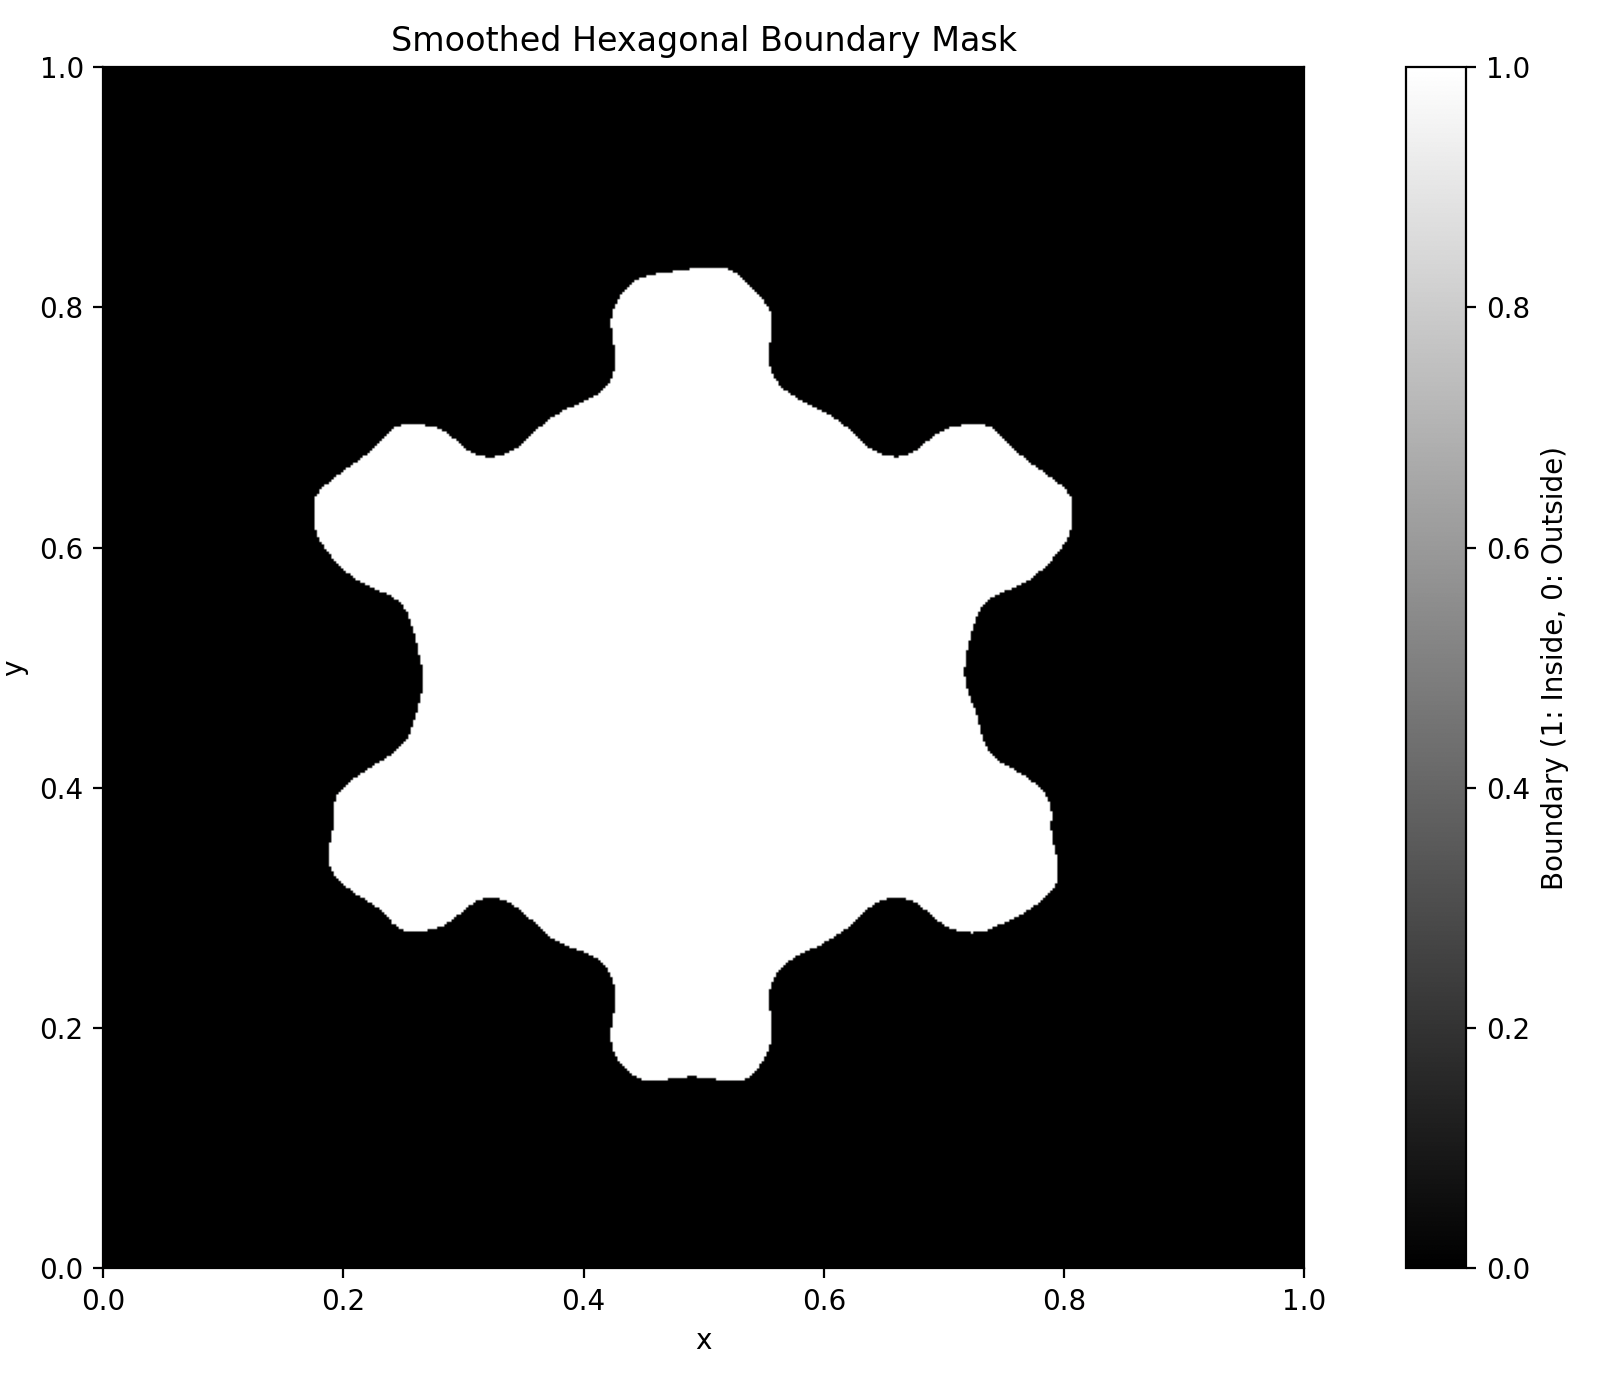
\includegraphics[height=.8\linewidth]{gaussian.png}
    \caption{Gaussian Convolution}
    \label{grad}
    \end{subfigure}
    \caption{融化模型}
    \label{pog}
\end{figure}
\begin{figure}[H]
\centering
\begin{subfigure}{.5\textwidth}
    \centering
    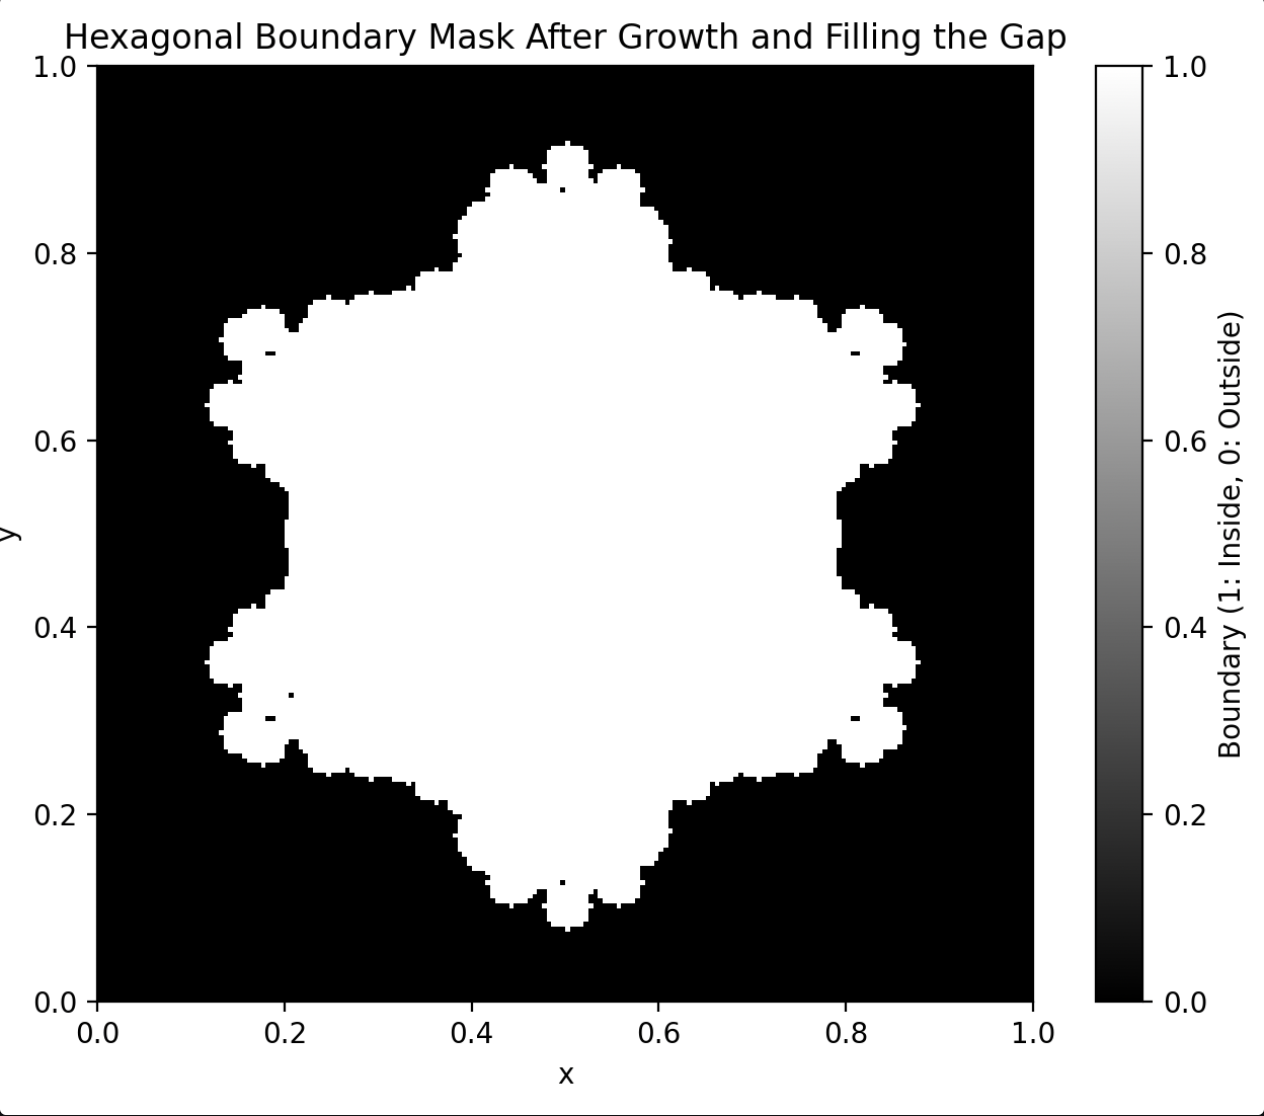
\includegraphics[height=.8\linewidth]{sphere.png}
    \caption{截斷模型}
    \label{pot}
\end{subfigure}%
\begin{subfigure}{.5\textwidth}
    \centering
    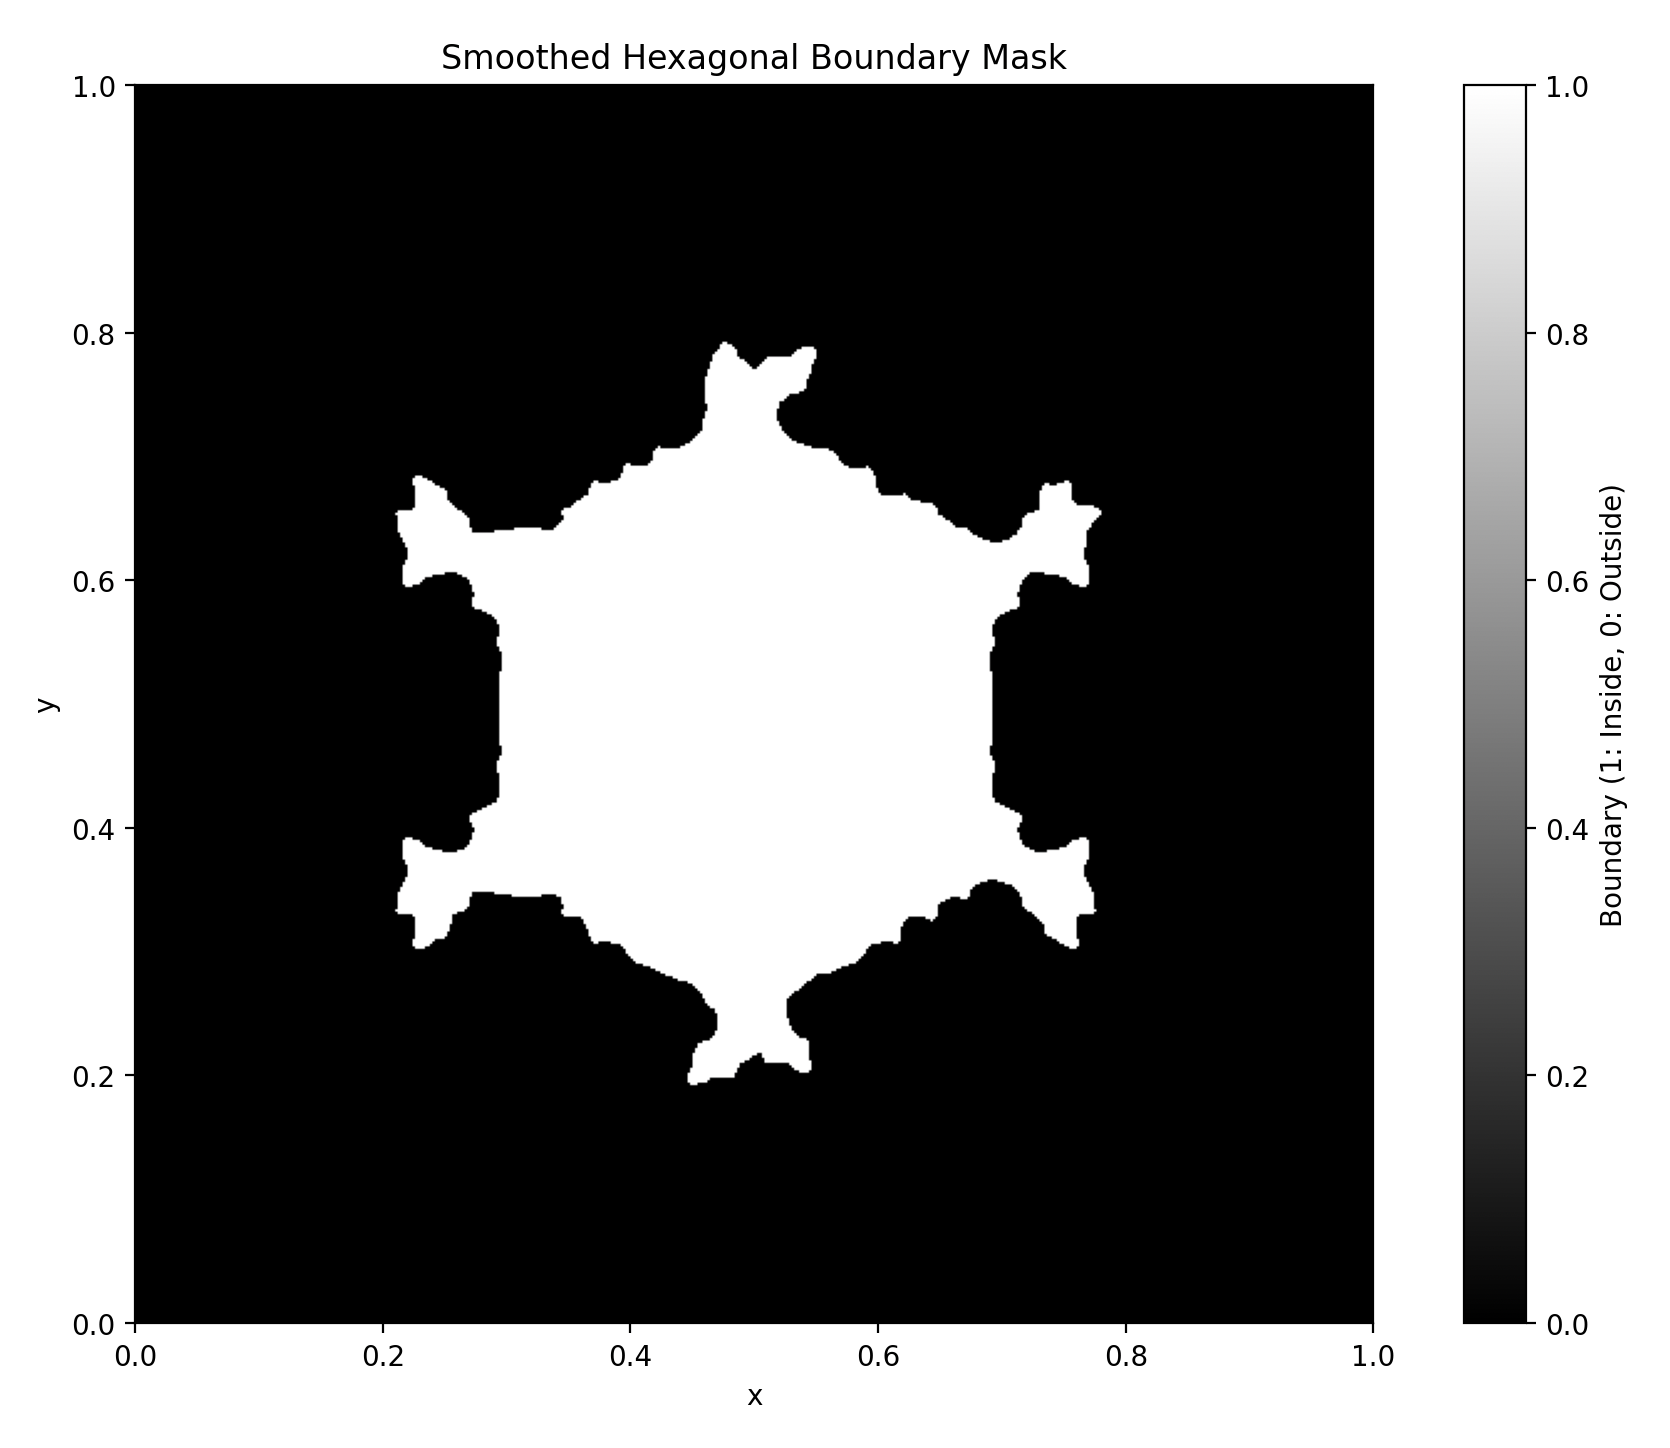
\includegraphics[height=.8\linewidth]{no_melt.png}
    \caption{無融化模型}
    \label{grad}
    \end{subfigure}
    \caption{融化模型}
    \label{pog}
\end{figure}

以上是四種融化模型給出的雪花,可以看出他們的共通點都是在尖端會長得特別多,而凹槽會特別少。由於此特性,六邊型的六角上的冰晶都特別多。但對於各不同模型仍有差別。可以看到這些模型大多無法做到像是傳統我們雪花的針狀結晶及一堆分岔,主要理由是我們的模型解析度過低,一但要解析這些針狀結晶便會有很大的困難,但是在Gaussian Convolution的模型下可以看見他的雪花的大致形狀比較符合我們的預期,而利用液滴模擬的模型則有比較好的分岔特性。利用截斷模型則可以看到部分的片狀成長特徵,但是由於數值問題在部分的點會有缺陷,導致空缺。不用融化模型的冰晶可以看到特別集中於尖端,但形狀完全非預期中的狀況。
\subsection{總結}
我們發現到我們的雪花模擬模型的確有符合基本的物理狀況,包括尖端成長較快及凹槽成長較慢。惟有在融化的模型上比較難掌握,部分模型掌握了大特徵,卻很難掌握細部特徵,但可以掌握細部特徵的模型又因為解析度不足而導致結果不甚合理,故若要有更好的預測必須引入更多參數和假設才能解決。本報告的程式細節將放在Github網址上。
\section*{References}
[1] Discrete Poisson equation, \url{https://en.wikipedia.org/wiki/Discrete_Poisson_equation}
[2] ChatGPT for code assisting
\end{document}
